\documentclass[main.tex]{subfiles} 
\begin{document}

\section*{Teoretisk bakgrunn}
Gjennom underveisvurderingen følges elevenes progresjon i faget over tid, og læreren får informasjon
om oppnådd kompetanse. Hensikten med slik vurdering er å gi et grunnlag for å forbedre og videreutvikle  
kvaliteten på opplæringen (NOU 2015:8, s. 92). I utredningen, \emph{NOU 2015:8 Fremtidens skole}, vektlegges
fagovergripende kompetanser, dvs. for eksempel lesing, skriving, utholdenhet, motivasjon, og å kunne planlegge, 
gjennomføre og vurdere egne læringsprosesser (NOU 2015:8, s. 66) :
\begin{displayquote}
Utvalget anbefaler at fagovergripende kompetanser vektlegges i fremtidens skole. Siden det  
anbefales å integrere dem i fagene, vil informasjon om elevenes kompetanse i fag være viktig.  
Samtidig vil skoler, skoleeiere og nasjonale myndigheter ha behov for informasjon om elevenes utvikling av 
prioriterte fagovergripende kompetanser, for å kunne bidra til at de vektlegges i opplæringen. 
(Ludvigsen-utvalget 2015)
\end{displayquote}
\citeA[s. 3]{smit09} beskriver hvordan vurderingslandskapet forandrer seg, fra internasjonale tester til
individuell fremoverføring. Gjennom \emph{vurderingslinjen} (se figur \ref{fig:smit09}) beskriver hun
\begin{figure}[h!]
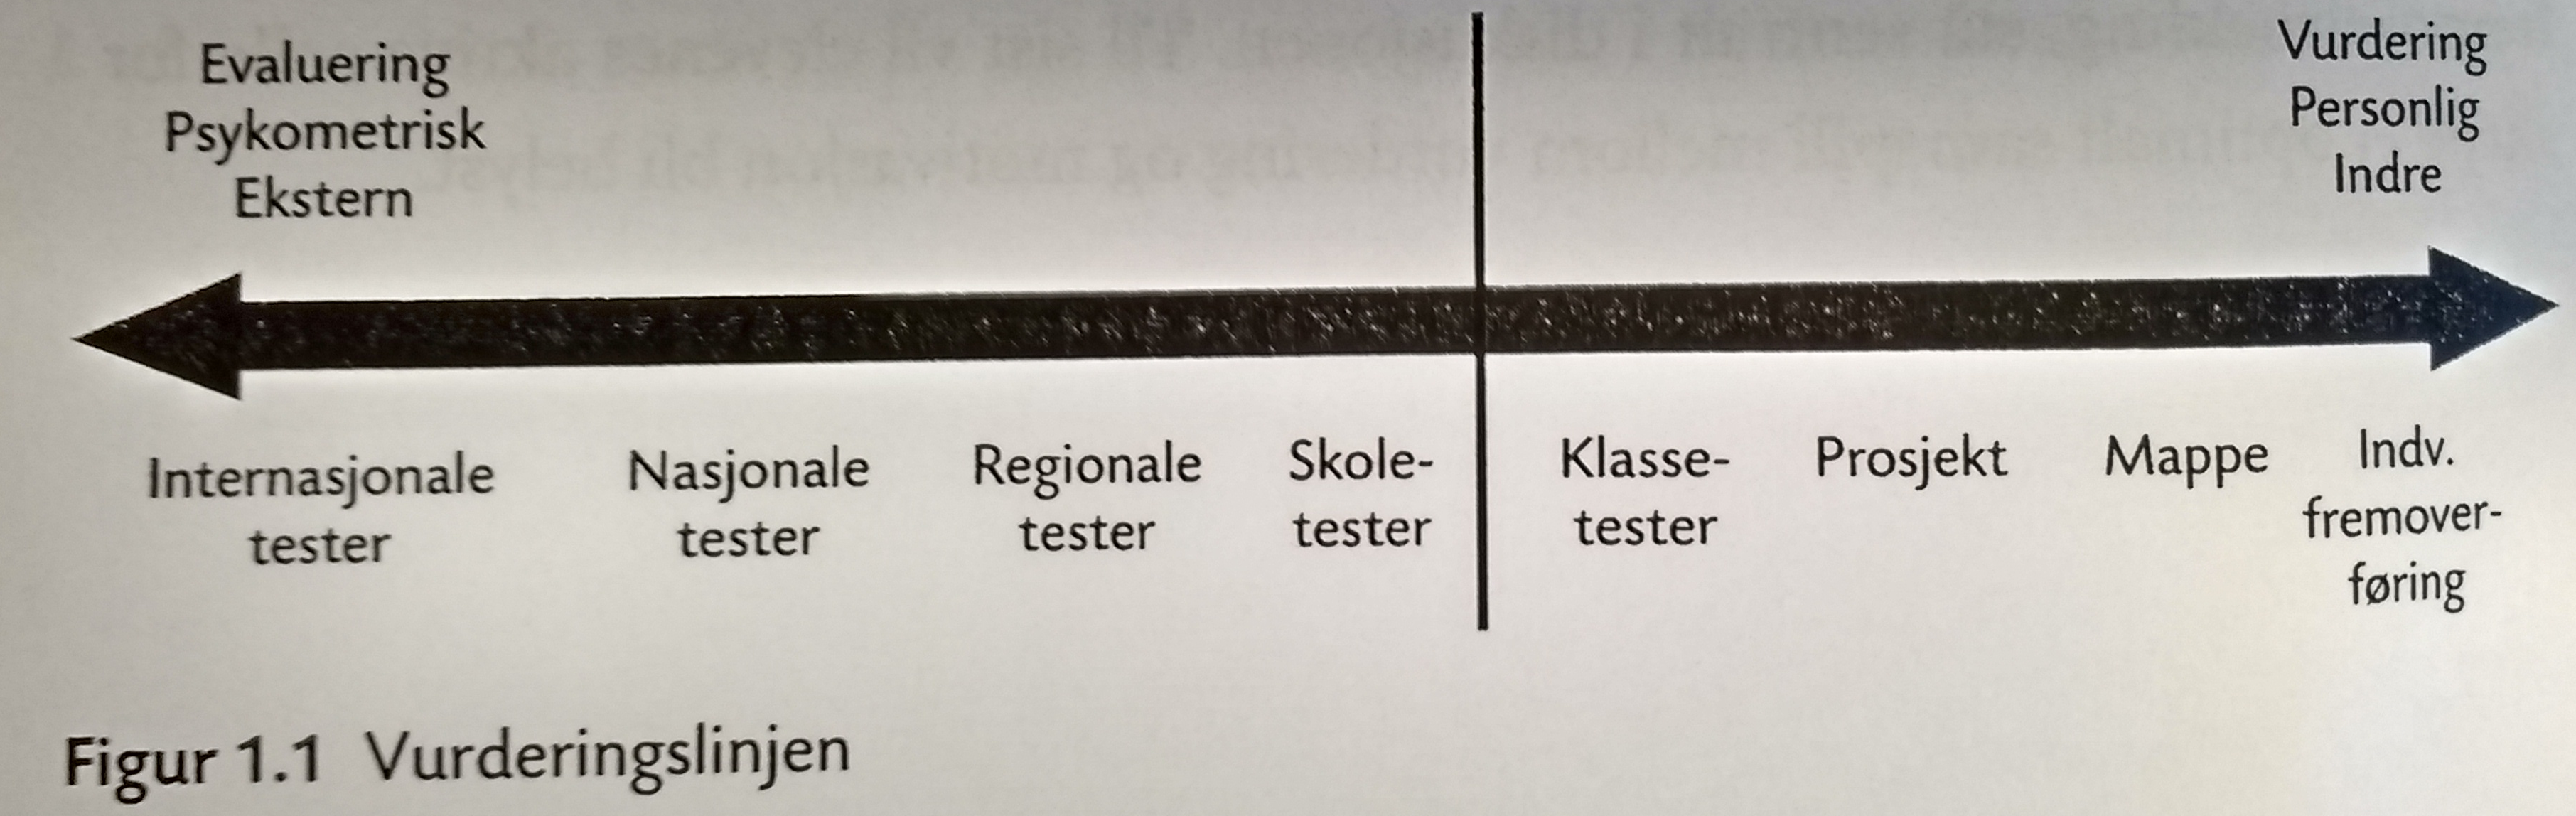
\includegraphics[scale = 0.1]{../figures/vurderingslinjen.png}
\caption{Vurderingslinjen. Kilde: \protect\citeA{smit09}.}
\label{fig:smit09}
\end{figure}

Skriv om : Summativ vs formativ vurdering
\newline
\newline
I læringsrettet vurdering stilles det strengere krav til lærerers evner som evaluator. Da er det viktig å se på lærerens læringssyn. 
Her er to eksempeler på forskjellige læringssyn :
\newline
\newline
\textbf{Læring som overføring av kunnskap}
\newline
I behavioristisk læringsteori foregår læring ved overføring av kunnskap, uavhengig av relasjonen mellom lærer 
og elev. Elev blir anskuet som et tomt kar, som det er lærerens jobb å fylle med kunnsakp. 
I et slikt læringssyn er vurdering i seg selv relativt ukomplisert, siden da gjelder det å 
formulere sine tilbakemeldinger på en så presis og elevtilpasset måte som mulig.
Derimot forventes det da at eleven tar til seg tilbakemeldingene og bruker dem til å rette seg etter.
Tilbakemeldingene vil da være begrenset til spesifikke svakheter relatert til faget eller kompetansemål.
Sentralt i behaviorismens syn på læring er betinging (\citeNP[s. 74]{salj13}). Ved ønsket atferd belønnes 
handlingen. Dette referes som forsterking (\citeNP[s. 22]{hell07}). Innenfor vurderingskontekten er
tilsiktet hensikt å motivere elevene. Dermed er karakteren en forsterker for noen og straff for andre.
\newline
\newline
\textbf{Læring som en relasjonell prosess}
\newline
Sett fra det relasjonelle perspektivet består det i å veilede elevene i den nærmeste utviklingssonen.
Den \emph{nærmeste utviklingssonen} beskriver en sone som ligger i mellom en elevs kognitive 
ferdigheter, dvs. hva de kan oppnå selvstendig uten hjelp, og elevens potensielle utvikling, dvs. 
hva en elev kan få til eller forstå gjennom veiledning (\citeNP[s. 125]{bta98}; \citeNP[s. 75]{salj13}). 
Bruk av ''scaffolding`` eller stillasbygging (\citeNP{bta98}) er da viktig for å knytte fagbegreper og teori til elevenes 
forkunnskaper. Vurderingsarbeidet vil derfor også gi den forskende lærer (\citeNP[s. 19]{hell07}) verdifull informasjon 
om sin egen didaktiske tilrettelegging.
Jeg vil komme tilbake til disse læringssyn når jeg evaluerer min egen praksis gjennom FoU arbeidet.
\newline
\newline
En av sentrale styringsrammene for norske utdanningspolitikk og skolepraksis er prinsippet om tilpasset opplæring.
Opplæringen skal ivareta sentrale verdier som inkludering, variasjon, sammenheng, relevans, verdsetting, medvirkning og 
erfaringer. Dette skal operasjonaliseres av undervisere gjennom differensiering.  Undervisningen må, ved hjelp av 
differensiering, tilfredsstille alle elevenes tilretteleggingsbehov i klassen, fra elever med matematikkvansker 
(dyskalkuli) til evnerike elever. Når en lærer jobber med elever hvor spennet er så pass stort, med andre ord at elevene 
utgjør en heterogen gruppe, da kan heller ikke undervisningen være homogenisert. Jeg kan derfor allerede nå påstå at en 
behavioristisk tilnærming til vurdering for læring vil tydeligvis ikke oppfylle prinsippet om tilpasset opplæring.
\begin{figure}[h!]
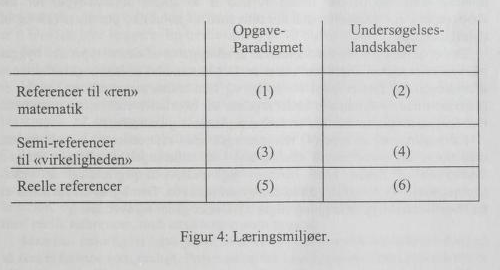
\includegraphics[scale = 0.9]{../figures/laeringsmiljoer.png}
\caption{Kilde: \protect\citeA{skov98}.}
\label{fig:skov98}
\end{figure}
I tabellen \ref{fig:skov98}, kartlegger \citeA{skov98} type oppgaver etter det han kaller \emph{oppgaveparadigmet} :
klassiske åpne og lukkede oppgaver vs. \emph{undersøgelseslandskaber} eller utforskende oppgaver. I tabellen tallfester
han disse oppgavetypene etter i hvilken grad de er tilnærmet virkeligheten. Jeg kommer til å bruke tabellen når jeg
drøfter oppgavene fra kartleggingsprøven (se vedlegg : \ref{sec:prove}).
\newline
\newline
Før vi forsetter videre er det lurt å bemerke noe termer jeg vil bruke videre i denne oppgaven.
\newline
Vurdering av læring
\newline
Vurdering for læring
\newline
Summativ vurdering
\newline
Fomativ vurdering
\newline
\newline
Å skrive matematikk regnes som en av grunnleggende ferdighetene. Det innebærer blant å beskrive og forklare 
egen tankgegang, å lage tegninger og skissere grafer. Skriving i matematikk blir sett på som et redskap for å 
utvikle egne tanker og egen læring (\citeNP{udirGF}).
\newline\newline
Pyskologene Daniel Kahneman og Amos Tversky har satt fram en teoretisk ramme for å undersøke læring av sannsynlighet og 
statistikk. Deres tese er at mennesker uten erfaring, refleksjon og innsikt i statistikk,
bruker følgende strategier for å bedømme sannsynlighet (\citeNP{udir13}; \citeNP{evan17}):
\begin{itemize}
\item Representativitet : små utvalg skal representere den fordelingen som finnes i populasjonen
\item Tilgjengelighet : sannsynlighet bedømmes ut fra hvor lett det er å huske spesielle tilfeller
\item Resultatorientering : utfallet kan forutses, som ved en deterministisk prosess
\item Konjunksjonsfellen : sannsynligheten for at to hendelser inntreffer samtidig er mindre enn sannsynligheten
for at en av hendelsene inntreffer.
\item Vanskeligheter med betinget sannsynlighet
\end{itemize}
\end{document}
